\section{Methods}

SNP array data from the Omni2.5 platform and sequence data from the HiSeq2000 platform was processed with PLINK v1.07\cite{Purcell2007} and \gls{GATK} v2.1 respectively unless otherwise noted. On page \pageref{subsec:chipQC} I describe the QC process for the SNP array data. On page \pageref{subsec:sequence} I describe the down sampling and the data curation of the sequencing data. On page \pageref{subsec:samplesize} I describe how we calculate an effective sample size at a fixed budget for each experimental method.



\subsection{SNP array QC}
\label{subsec:chipQC}

The populations were genotyped on either the Illumina HumanOmni2.5-4 (quad) or -8 (octo) platforms. Table \ref{tab:chips_preQC_summary} summarizes the content of each chip prior to QC. Table \ref{tab:chip_sample_summary} summarizes the samples genotyped and called on each platform.
\begin{table}[htp]
\centering
\begin{tabular}{l|rr}
\hline
               & HumanOmni2.5-4 & HumanOmni2.5-8 \\ \hline
All            & 2,450,000      & 2,379,855      \\ \hline
               &                &                \\
Autosomal 1-22 & 2,390,395      & 2,314,174      \\
X              & 57,061         & 55,208         \\
Y              & 1,897          & 2,561          \\
PAR            & 554            & 418            \\
Mitochondrial  & 93             & 256            \\
Unplaced       & 0              & 7,238          \\ \hline
\end{tabular}
\caption{Summary of SNPs on each the two SNP arrays.}
\label{tab:chips_preQC_summary}
\end{table}
\begin{table}[h]
\centering
\begin{tabular}{lllll}
\hline
Project  & \multicolumn{2}{l}{AGVP} & uganda\_gwas & HiSeq intersection \\ \hline
Platform & quad        & octo       & octo         &                    \\ \hline
Zulu     & 9           & 95         & 0            & 95                 \\
Baganda  & 90          & 197        & 3585         & 94                 \\
Ethiopia & 0           & 108        & 0            & 63                
\end{tabular}
\caption{Sample counts for the 3 African populations after QC. The QC process was slightly different for the Baganda samples.}
\label{tab:chip_sample_summary}
\end{table}

The \gls{QC} was carried out with PLINK 1.07\cite{Purcell2007}, Python 3\footnote{\url{https://www.python.org}} and the GNU core utilities\footnote{\url{https://www.gnu.org/software/coreutils}}. We removed samples without proper consent prior to genotype calling. Genotype calling was carried out with the Illuminus algorithm at the \gls{WTSI}. Three sets were called independently; i.e. 4892 Ugandan samples on the octo platform and additional African samples on the quad and octo platforms (see supplementary table 3 on page 5 of the supplementary material of the \gls{AGV} project publication\cite{Gurdasani2015}). Prior to the \gls{QC} we updated genders for samples with genotype gender issues as determined by PLINK in accordance with new data collection of genders. The QC was slightly different for the 5000 Ugandan samples (appendix \ref{app:qc_uganda_gwas}) of which approximately two thirds were Baganda. Specifically we used a lower \gls{HWE} probability threshold of $10^{-8}$ instead of a lower threshold of $10^{-6}$. This was because the Ugandan samples were highly related and we expected more deviations from \gls{HWE}. For the same reason we applied an \gls{IBD} threshold of 0.9 instead of 0.05. We used sample and \gls{SNP} call proportions of 0.97 instead of 0.98 for the Ugandan samples. We also expect the genotype calls to be better for larger sample sizes, which would allow for a more stringent \gls{QC}, but we never evaluated this. The \gls{QC} for the two other main datasets, which was carried out per population and per platform, is described in the following sub sections. The \gls{QC} of the Uganda \gls{GWAS} data set is described in the appendix on page \pageref{app:qc_uganda_gwas}.

\subsubsection{Harmonisation of .strand files}
The .strand file contains information on how to flip alleles from Illumina TOP alleles to the forward strand. The purpose of the harmonisation of the .strand files is to obtain a single clean strand file containing only SNPs common to both original strand files. A summary of the original .strand files is given in table \ref{tab:strand_files}.
\begin{table}[h]
\centering
\begin{tabular}{l|rr}
\hline
                       & quad      & octo      \\ \hline
Build                  & 36        & 37        \\
Total SNP count        & 2,449,906 & 2,379,514 \\
Autosomal SNP count    & 2,388,854 & 2,320,543 \\
Chromosome X SNP count & 57,623    & 55,902   
\end{tabular}
\caption{Description of the original .strand files.}
\label{tab:strand_files}
\end{table}

First we updated the positions in the quad (Omni2.5-4) .strand file from \gls{GRCh}\cite{10.1371/journal.pbio.1001091} build 36 to build 37 using liftOver.\cite{Karolchik01012014} SNPs that failed to be remapped were excluded. After updating the build we removed \glspl{SNP} in the .miss and the .multiple files from the quad and octo (Omni2.5-8) .strand files; the .miss file contains \glspl{SNP} that did not reach the required threshold for mapping to the genome and the .multiple file contains \glspl{SNP} that had more than 1 high quality match to the genome. For each position in the .multiple file we exclude all but one of the \glspl{SNP}.
After updating the build and removing \glspl{SNP} in the .miss and .multiple files we removed duplicate coordinates from the .strand file. We preferably kept the reference \gls{SNP}.
\footnote{\url{http://www.ncbi.nlm.nih.gov/SNP/get_html.cgi?whichHtml=how_to_submit\#REFSNP}} In the absence of a reference SNP the first record was kept. If both positions corresponded to reference SNPs, then the first one was kept.
Afterwards we excluded \glspl{SNP} not present in both .strand files; i.e. we required the coordinate and the alleles to be identical. The SNP exclusion from the strand files is summarized in table \ref{tab:strand_file_exclusion_summary}.
\begin{table}[h]
\centering
\resizebox{\textwidth}{!}{%
\begin{tabular}{ll|rrr|rrr}
\hline
                                                                    &              & \multicolumn{3}{c}{Omni2.5-4}    & \multicolumn{3}{c}{Omni2.5-8}            \\
Filtering step                                                      & Chromosome   & Before    & Filtered & After     & Before       & Filtered    & After       \\ \hline
\multirow{3}{*}{Update from build 36 to build 37}                   & All          & 2,449,906 & 1,890    & 2,448,016 & \multicolumn{3}{c}{\multirow{3}{*}{N/A}} \\
                                                                    & Autosomal    & 2,388,854 & 327      & 2,388,527 & \multicolumn{3}{l}{}                     \\
                                                                    & Chromosome X & 57,623    & 6        & 57,617    & \multicolumn{3}{l}{}                     \\ \hline
\multirow{3}{*}{Exclusion of SNPs in the .miss and .multiple files} & All          & 2,448,016 & 39,714   & 2,408,302 & 2,379,514    & 44,559      & 2,334,955   \\
                                                                    & Autosomal    & 2,388,527 & 36,465   & 2,352,062 & 2,320,543    & 40,391      & 2,280,152   \\
                                                                    & Chromosome X & 57,617    & 2,429    & 55,188    & 55,902       & 2,853       & 53,049      \\ \hline
\multirow{3}{*}{Exclusion of duplicates}                            & All          & 2,408,302 & 9,510    & 2,398,792 & 2,334,955    &             & 2,379,514   \\
                                                                    & Autosomal    & 2,352,062 & 6,794    & 2,345,268 & 2,280,152    & 3,148       & 2,277,004   \\
                                                                    & Chromosome X & 55,188    & 2,715    & 52,473    & 53,049       & 2,424       & 50,625      \\ \hline
\multirow{3}{*}{Exclusion of SNPs not common to the .strand files}  & All          & 2,398,792 & 88,876   & 2,309,914 & 2,329,381    & 19,465      & 2,309,914   \\
                                                                    & Autosomal    & 2,345,268 & 86,948   & 2,258,318 & 2,277,004    & 18,684      & 2,258,318   \\
                                                                    & Chromosome X & 52,473    & 1,906    & 50,567    & 50,625       & 58          & 55,902      \\ \hline
\end{tabular}
}
\caption{Summary of exclusions from strand files for all chromosomes, autosomes and the X-chromosome.}
\label{tab:strand_file_exclusion_summary}
\end{table}

\subsubsection{Harmonisation of data (.bim and .bed) files}
From the quad and octo \gls{SNP} array genotype data we removed rsIDs not present in the processed strand files. For the quad it was necessary to use the harmonized strand file with the original quad nomenclature as doing otherwise would create duplicate rsIDs. We updated the quad positions and rsIDs. SNPs that failed to be remapped were excluded. After updating the quad rsIDs we flipped the quad and octo \glspl{SNP} to the forward strand according to the processed .strand files. Finally we extracted \glspl{SNP} common between .strand and .bim files and common between the quad and octo .bim files. The SNP exclusion from the genotype data files is summarized in table \ref{tab:bim_file_exclusion_summary}.
\begin{table}[h]
\centering
\resizebox{\textwidth}{!}{%
\begin{tabular}{ll|rrr|rrr}
\hline
                                                                            &              & \multicolumn{3}{c}{Omni2.5-4}    & \multicolumn{3}{c}{Omni2.5-8}            \\
Filtering step                                                              & Chromosome   & Before    & Filtered & After     & Before       & Filtered    & After       \\ \hline
\multirow{3}{*}{Exclusion of SNPs missing in .strand files}                 & All          & 2,450,000 & 140,086  & 2,309,914 & 2,379,855    & 69.941      & 2,309,914   \\
                                                                            & Autosomal    & 2,390,395 & 132.078  & 2,258,317 & 2,314,174    & 61,235      & 2,252,939   \\
                                                                            & Chromosome X & 57,061    & 6,905    & 50,156    & 55,208       & 5,145       & 50,063      \\ \hline
\multirow{3}{*}{Update from build 36 to build 37}                           & All          & 2,309,914 & 412      & 2,309,502 & \multicolumn{3}{c}{\multirow{3}{*}{N/A}} \\
                                                                            & Autosomal    & 2,258,317 & 1        & 2,258,316 & \multicolumn{3}{l}{}                     \\
                                                                            & Chromosome X & 50,156    & 0        & 50,156    & \multicolumn{3}{l}{}                     \\ \hline
\multirow{3}{*}{Exclusion of SNPs not common to all data and .strand files} & All          & 2,309,502 & 7,139    & 2,302,363 & 2,309,914    & 7,551       & 2,302,363   \\
                                                                            & Autosomal    & 2,258,316 & 7,001    & 2,251,315 & 2,252,939    & 1,624       & 2,251,315   \\
                                                                            & Chromosome X & 50,156    & 136      & 50,020    & 50,063       & 43          & 50,020      \\ \hline
\end{tabular}
}
\caption{Summary of exclusions from bim and bed files of SNPs on all chromosomes, autosomes and the X chromosome.}
\label{tab:bim_file_exclusion_summary}
\end{table}

\subsubsection{QC steps after harmonisation of files}
The data was split by population and platform (i.e. quad and octo) and \gls{QC} was carried out for individual data sets. The \gls{QC} that was carried out for each population is described elsewhere.\cite{Gurdasani2015} All steps except heterozygosity calculations and IBD sample pruning were carried out with PLINK; heterozygosity calculations are erroneous for PLINK and PLINK cannot do \gls{IBD} sample pruning, which is an \gls{NP}-complete problem. Instead we used Python for these tasks.\footnote{\url{https://github.com/team149/tc9/blob/master/QC/QC_IBD_prune.py}} In summary the QC consisted of sequential checks of
\begin{enumerate}
\item Sample call proportion (>0.98)
\item Heterozygous proportion (\textless $\pm$ 3\glspl{SD})
\item Gender (F>0.8 males, F<0.2 females)
\item SNP call proportion for the autosomes (\textgreater0.98)
\item IBD (<0.05)
\item SNP call proportion for the X chromosome (\textgreater0.98)
\item \gls{HWE} (\textit{p}$_{HWE}$<10$^{-6}$) on all autosomal SNPs and female X chromosome SNPs.
\end{enumerate}



\subsection{Curation of original and down-sampled sequence data}
In addition to carrying out \gls{QC} of the \gls{SNP} array data, we also did data curation of the low coverage and \gls{ULC} sequence data for the 3 populations. A flow diagram illustrating the variant calling process and further data processing is shown in figures \ref{fig:SN09f1} and \ref{fig:SN12f1}.
\begin{figure}
\centering
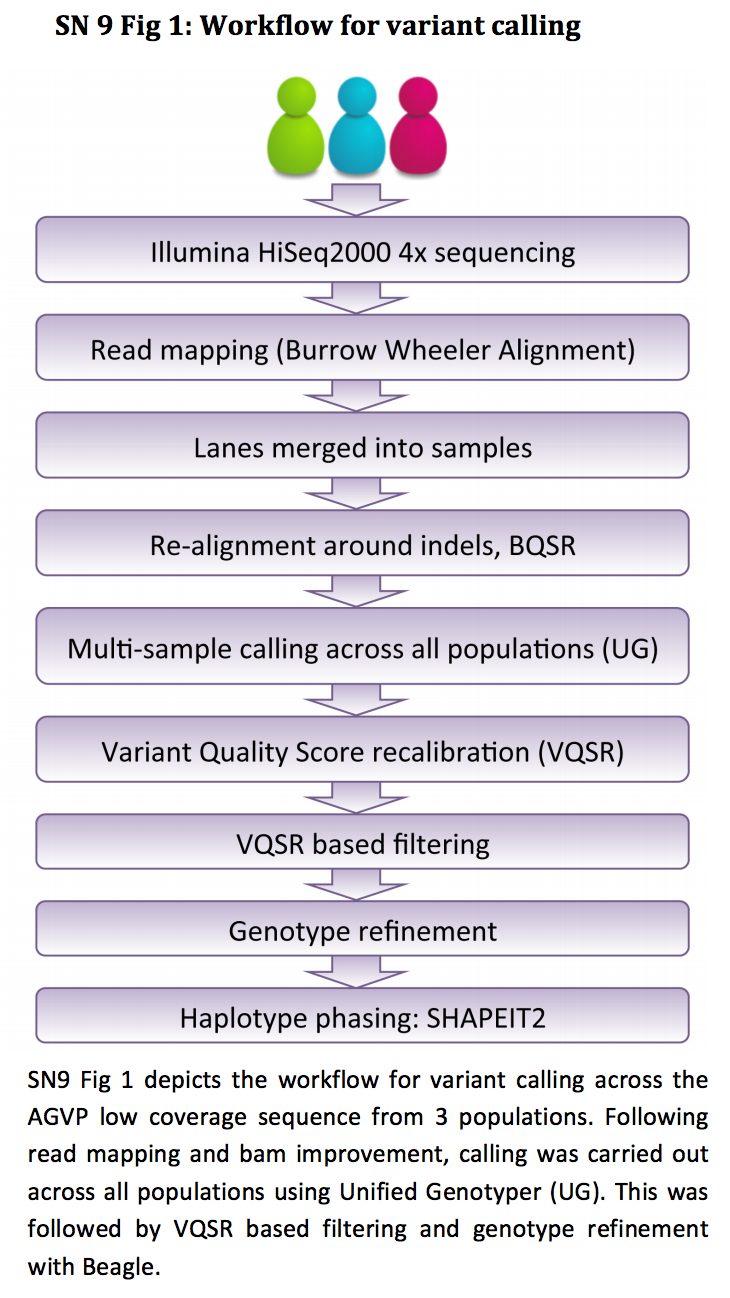
\includegraphics[trim={0 4.25cm 0 0.75cm},clip,width=0.66\textwidth]{fig/SN09f1}
\caption[Variant calling flow diagram.]{Work flow for variant calling across the low coverage \gls{WGS} data from 3 populations. Following read mapping and bam improvement, calling was carried out across all populations using \gls{UG}. This was followed by \gls{VQSR} based filtering with \gls{GATK} and genotype likelihood refinement with Beagle. Figure created by Deepti Gurdasani.}
\label{fig:SN09f1}
\end{figure}

The data curation process after sequencing involves mapping of reads to the reference genome, \gls{BAM} file pre-processing, variant calling, variant filtering, genotype likelihood refinement and phasing to obtain haplotypes.

The data is also down-sampled to lower coverage prior to \gls{BAM} file pre-processing for the purpose of identifying the most cost effective study design. Specifically the data was randomly down-sampled to 0.5x, 1x and 2x coverage using \href{https://www.broadinstitute.org/gatk/gatkdocs/org_broadinstitute_gatk_tools_walkers_readutils_PrintReads.php}{GATK PrintReads} as described on page \pageref{subsubsec:downsampling} prior to pre-processing of the raw reads.

A flow diagram explaining the curation of \gls{WGS} data down-sampled to lower coverage and the comparison with \gls{WGS} data at higher coverage and imputed SNP array data is shown in figure \ref{fig:SN12f1}. The down-sampling is carried out prior to pre-processing of raw reads after initial alignment as described in detail on page \pageref{subsubsec:downsampling}.
\begin{figure}
\centering
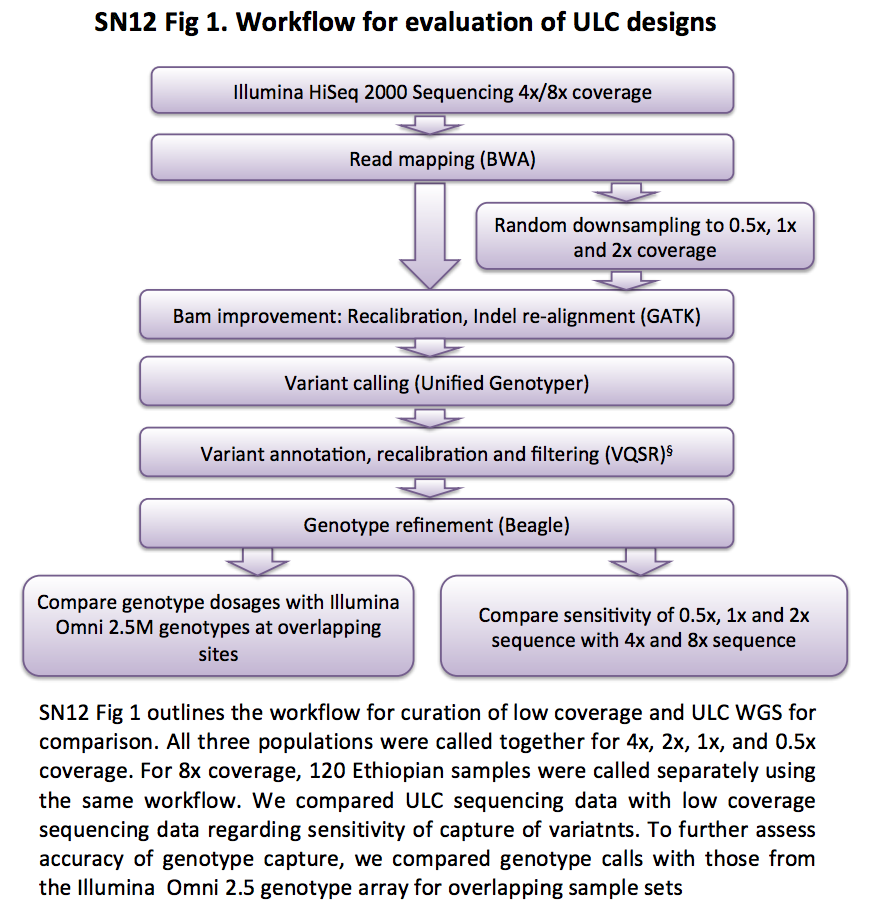
\includegraphics[trim={0 4cm 0 1cm},clip,width=0.8\textwidth]{fig/SN12f1}
\caption[Work flow for evaluation of \gls{ULC} designs.]{Flow diagram for curation and comparison of low coverage and \gls{ULC} \gls{WGS} data. All three populations were called together for 4x, 2x, 1x, and 0.5x coverage. For 8x coverage, 120 Ethiopian samples were called separately using the  same  work flow. \gls{ULC} sequencing data was compared with low coverage sequencing data regarding ability to capture variants; i.e. sensitivity. To further assess accuracy of genotype capture, genotype calls were compared with those from the Illumina Omni 2.5 genotype array for overlapping sample sets. Figure created by Deepti Gurdasani.}
\label{fig:SN12f1}
\end{figure}

\subsubsection{Sequencing}
\label{subsec:sequence}
Sequence data for the same SNP array genotyped populations was also generated (table \ref{tab:sequence_sample_summary}). Blood samples were collected by local collaborators. Library preparation and sequencing on Illumina HiSeq2000 machines were carried out at the \gls{WTSI} by \gls{HGI}.

\begin{table}[h]
\centering
\begin{tabular}{l|ll}
Population & Count & Omni intersection \\ \hline
Baganda    & 100   & 94                \\
Zulu       & 100   & 95                \\
Ethiopia   & 120   & 63               
\end{tabular}
\caption{Count of sequenced samples and overlap with SNP array genotyped sample sets.}
\label{tab:sequence_sample_summary}
\end{table}

\subsubsection{QC of raw reads}
In order to ensure the quality of the raw reads produced for the project, an automatic \gls{QC} system was employed by \gls{HGI} at the \gls{WTSI} to reduce the number of data files that required manual intervention. This system was been derived from the one originally designed for the UK10K project and uses a series of empirically derived thresholds to assess summary metrics calculated from the input \glspl{BAM}. These thresholds include: percentage of reads mapped; percentage of duplicate reads marked; various statistics measuring indel distribution against read cycle and an insert size overlap percentage. Any lanes that fell below the "fail" threshold for any of the metrics were excluded; any lanes that fell below the "warn" threshold on a metric were manually examined; and any lane that did not fall below either of these thresholds for any of the metrics was given a status of "pass" and allowed to proceed into the later stages of the pipeline.

\subsubsection{Downsampling to lower coverage}
\label{subsubsec:downsampling}
Downsampling to a lower coverage was carried out to enable comparison of ultra low coverage study designs with low coverage and SNP array study designs. Samples were downsampled to average coverages of 8x, 4x, 2x, 1x and 0.5x. Downsampling was carried out on the raw reads converted to lanelet bam files prior to pre-processing to best simulate a real case scenario. Instead of downsampling by unit fractions\cite{10.1371/journal.pcbi.1002604}, downsampling was carried out to achieve a specific integer value coverage across all samples in a given population. The downsampling fraction (equation \ref{eq:downsampling}) was calculated from the initial coverage across all samples, which was calculated from the number of mapped reads, which was counted with samtools\cite{Li15082009} flagstat. The read length on the Illumina HiSeq2000 is 100. We divided by the number of non N bases in the reference genome (2.85\gls{Gbp}) to which reads can be mapped.

\begin{equation}
\text{downsampling factor} =  \frac
{\text{read length} \times \text{count of mapped reads}}
{\text{desired coverage} \times \text{genome size} \times \text{count of samples}}
\label{eq:downsampling}
\end{equation}

Downsampling to a lower coverage was carried out with \gls{GATK}Lite2.1 PrintReads.\cite{DePristo2011}\footnote{For the Baganda dataset downsampled to 2x \gls{GATK}2.5 was used, because our data was deleted by mistake.}
%Avoiding read mapping bias was not ensured by sorting the reads by read name before downsampling and resorting the downsampled reads by coordinate.
After down-sampling the reads were realigned and recalibrated as described in the next section.

\subsubsection{Pre-processing of raw reads}
We carried out downsampling of the raw reads to a lower coverage prior to pre-processing. The following pre-processing steps for the 100bp length reads stored in .bam files was carried out in sequence:
\begin{enumerate}
\item Marking of duplicates on a lanelet level with Picard MarkDuplicates.
\item Mapping of reads to \gls{GRCh} 37 with decoys using BWA-backtrack\cite{Li15072009} designed for Illumina sequence reads up to 100bp.
\item Merging of lanelets that pass \gls{QC} into sample level files with Picard MergeSamFiles.
\item Marking of duplicates on a sample level with Picard MarkDuplicates.
\item Re-alignment around known and discovered indels with \gls{GATK} RealignerTargetCreator and IndelRealigner. Known indels for realignment were taken from the Mills Devine and \gls{1000G} Gold set and the 1000G phase 1 low coverage set.
\item \Gls{BQSR} with \gls{GATK} BaseRecalibrator and PrintReads. Known variants for \gls{BQSR} were taken from dbSNP 137.
\item Creation of "MD" tag with samtools calmd and indexing.
\end{enumerate}

We mark duplicates for exclusion, because sequencing errors are otherwise propagated in duplicates leading to false positive variant calls. Base quality doesn't have any impact on indel realignment, but having reads realigned properly improves the base recalibration model, because it reduces the number of artifactual \glspl{SNP}. It supposedly improves accuracy of downstream processing steps. This assumption was never tested.
%Recommendations here: https://www.broadinstitute.org/gatk/guide/article?id=1247

\subsubsection{Variant Calling}
We evaluated different variant calling software packages. We decided to use \gls{GATK} \gls{UG}. It has an ability to call more \glspl{SNP} with a quality above 4 than any other variant caller (figure \ref{fig:venn4_varcall_Platypus_filter_QUAL4_incl_MNPs_TiTv}). We did not evaluate whether all of the called variants were true positives, but we did take note of the variants unique to \gls{UG} having a relatively high \gls{TiTv} ratio, which indicates that the variants could be true positives. Furthermore the variant count was carried out prior to filtering, which would further filter out false positives. Hence a high sensitivity at this stage is preferable. If more time had been available, then we would have calculated the sensitivity and specificity for each variant caller by comparison to a truth set. We would also have evaluated indel calling abilities.

\begin{figure}[htb]
\centering
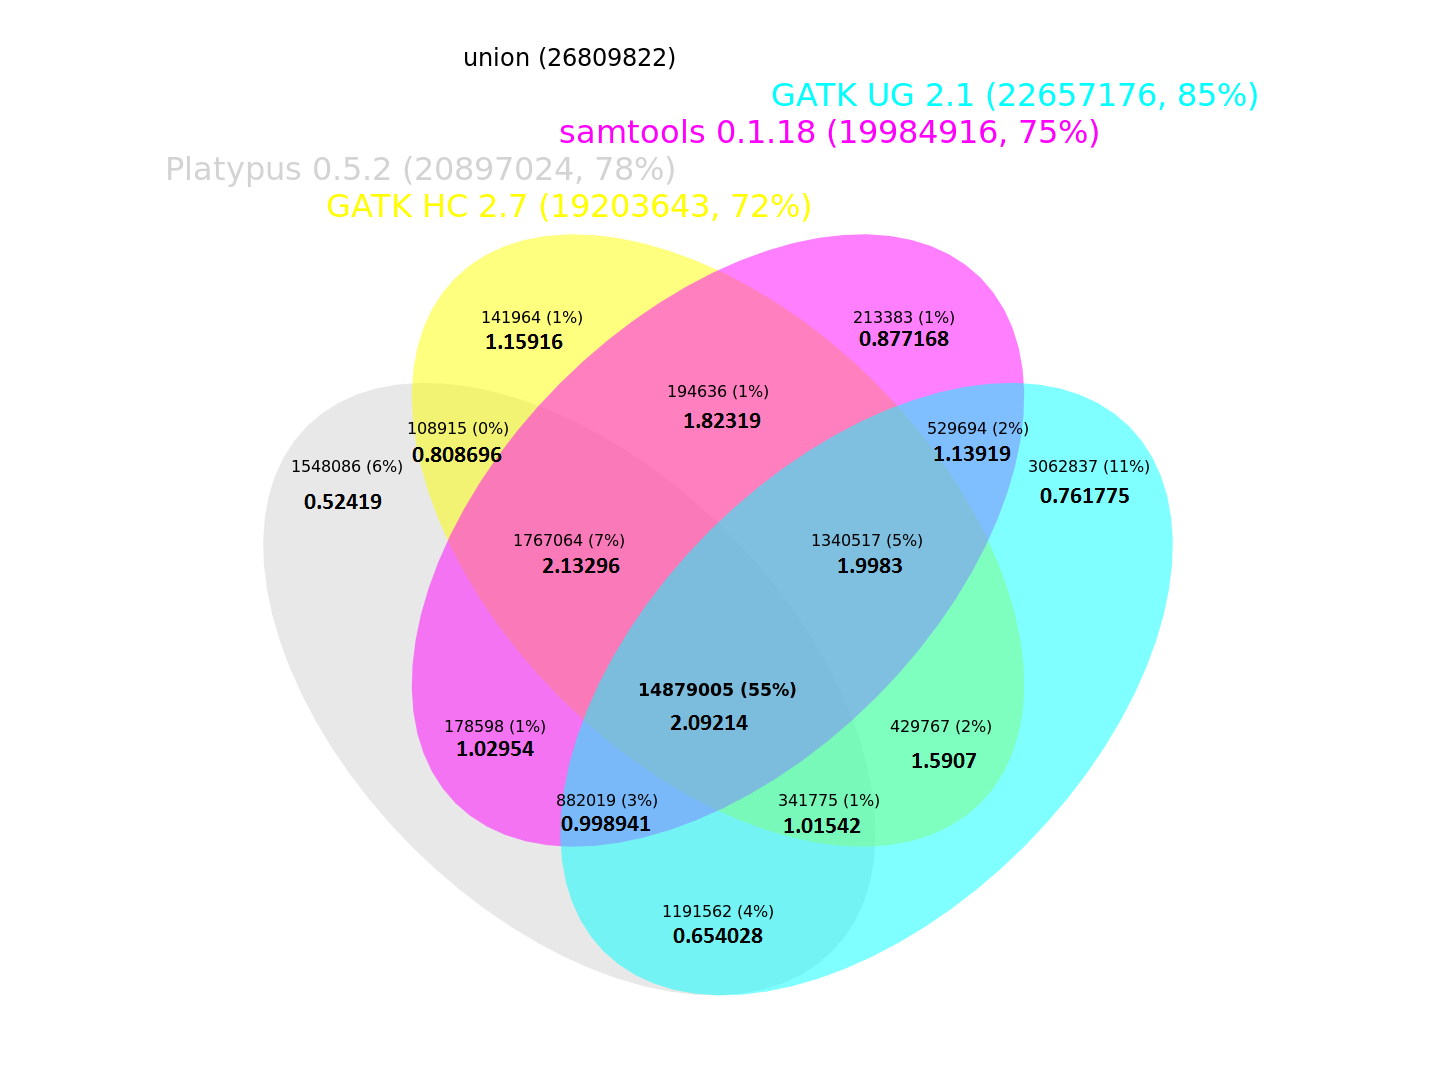
\includegraphics[width=0.8\textwidth]{fig/venn4_varcall_Platypus_filter_QUAL4_incl_MNPs_TiTv}
\caption{Comparison of variant callers. SNPs and MNPs were called with four different variant callers from Baganda 4x sequence data. A quality threshold of 4 was applied. The small numbers show the count of variants in each Venn set and the size of each set as a percentage of the size of the union set is printed in a parenthesis. The larger number in bold is the Ti/Tv ratio in each set. Platypus has a high sensitivity compared to the union set, but the variants unique to Platypus have a low Ti/Tv ratio, which indicates that they are false positives. \gls{GATK} \gls{UG} despite having a great number of unique variants has a higher Ti/Tv ratio than Platypus.}
\label{fig:venn4_varcall_Platypus_filter_QUAL4_incl_MNPs_TiTv}
\end{figure}

Variants were called in interval sizes of 10\gls{Mbp} without taking into consideration positions of centromeres and telomeres and density of variants. This impairs the ability to call variants at the end of regions and renders it impossible to call indels spanning two fragments. We accept this given the infinitesimally small read lengths compared to the much larger interval sizes.

Because of the shallow coverage (\textless 10x coverage per sample) and the small
number of samples we changed the default Phred quality score threshold at which variants should be called and emitted from 30 to 4 or 10 depending on the number of samples as per the \gls{GATK} GuideBook\footnote{page 13 of \url{https://www.broadinstitute.org/gatk/guide/pdfdocs/GATK_GuideBook_2.7-4.pdf}}. Otherwise we used default parameter values and default filters, which are described in the documentation of \gls{UG}\footnote{\url{https://www.broadinstitute.org/gatk/gatkdocs/org_broadinstitute_gatk_tools_walkers_genotyper_UnifiedGenotyper.php}}; i.e.
\begin{itemize}
\item \-\-downsampling\_type BY\_SAMPLE
\item \-\-downsample\_to\_coverage 250
\item \-\-min\_base\_quality\_score 17
\item \-\-max\_alternate\_alleles 6
\item DuplicateReadFilter to filter out duplicate reads.
\item UnmappedReadFilter to filter out unmapped reads.
\item MappingQualityUnavailableFilter to filter out reads with a mapping quality of zero.
\item BadMateFilter to filter out reads whose mate maps to a different contig.
\end{itemize}

For the final variant calling prior to the generation of the reference panel and simulation of the SNP array we did not include the samples NA12878 and NA19240 in the joint variant calling. This was to avoid bias in annotations used for filtering and to avoid inclusion of variants unique to either or both of the two samples.

Only the 120 Ethiopian samples were sequenced to 8x (table \ref{tab:samples} on page \pageref{tab:samples}). This dataset was therefore called separately unlike the lower coverage datasets, which were called across all samples.

\subsubsection{Variant Filtering}
The Gaussian mixture model of \gls{GATK} \gls{VR} was used for filtering called variants. The machine learning method was run simultaneously across all autosomes. The filtering is based on a \gls{VQSLOD} score, which is the log odds ratio of being a true variant versus being false under the trained Gaussian mixture model. The annotations we used for the model were
\begin{itemize}
\item Total depth over all samples (Coverage in versions prior to 2.4)
\item Phred-scaled p-value using Fisher’s exact test to detect strand bias (FisherStrand)
\item Consistency of the site with two segregating haplotypes (HaplotypeScore)
\item U-based z-approximation from the Mann-Whitney rank sum test for mapping qualities (MQRankSum)
\item Variant confidence divided by unfiltered depth of non-reference samples (QualByDepth)
\item Root mean square of the mapping quality of the reads across all samples (RMSMappingQuality)
\item U-based z-approximation from the Mann-Whitney rank sum test for the distance from the end of the read for reads with the alternate allele (ReadPosRankSumTest)
\end{itemize}

We used truth and training datasets with prior probabilities in accordance with best practices at the time (table \ref{tab:vr_sets}). The set of varints in \gls{dbSNP}\cite{Wheeler01012007} were used to determine the \gls{TiTv} ratio for known and novel variants. The novel \gls{TiTv} ratio was found to be very dependent on the version of \gls{dbSNP} used. Therefore we used a truth sensitivity threshold of 96\% while exploring the optimal variant calling method, which corresponded to a \gls{TiTv} ratio of 2.1, when using version 135 of \gls{dbSNP}. This threshold, which was lower than later best practises, ensured a high specificity at the cost of a lower sensitivity.
\begin{table}[h]
\centering
\begin{tabular}{lllll}
              & Known & Training & Truth & Prior Probability \\
HapMap 3.3    & False & True     & True  & 15                \\
1000G Omni2.5 & False & True     & False & 12                \\
dbSNP 135     & True  & False    & False & 8                
\end{tabular}
\caption{SNP sets used for training of the \gls{VQSR} model an d determination of known and novel counts.}
\label{tab:vr_sets}
\end{table}

We carried out a comparison of variant calling and variant filtering strategies. Specifically we tried doing variant calling and filtering within and across the 3 sequenced populations. We found that variant calling and filtering across the cohorts yields the greatest number of variants intersecting with the SNP array data.

After deciding on the best variant calling approach we wanted to decide on an optimal truth sensitivity threshold. For this purpose we included the 1000G samples NA12878 (\gls{CEU}) and NA19240 (\gls{YRI}) in the joint variant calling. The two samples have been sequenced by Complete Genomics\cite{Drmanac01012010} and Illumina\footnote{http://www.illumina.com/platinumgenomes/} to high coverage. We chose these samples, because a highly curated set of variant calls exist for NA12878\cite{Zook2014} and because NA19240 is an African sample. The reads we included in the joint variant calling were low coverage from the 20121211 release of 1000G; i.e. NA12878 at 6.4x and NA19240 at 4.1x. We chose a truth sensitivity threshold based on a \gls{ROC} curve sorted by \gls{VQSLOD} values (figure \ref{fig:SN09f2}). Ultimately we decided on a threshold of 99\%, which corresponds to a sensitivity of 88\%. This was also in accordance with \gls{GATK} best practices at the time.
\begin{figure}[htbp]
\centering
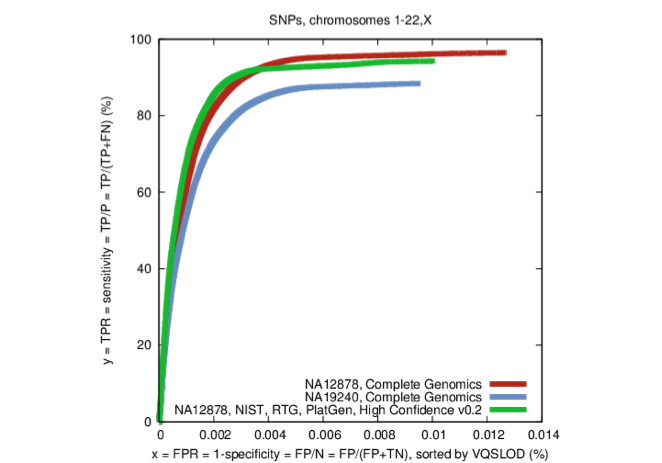
\includegraphics[width=0.8\textwidth]{fig/SN09f2}
\caption[\Gls{ROC} curve]{\gls{ROC} curve of low coverage \gls{WGS} data for NA12878 and NA19240 compared to 30x coverage sequencing for different \gls{VQSLOD} filtering scores. On the x-axis is the \gls{FPR} (1-specificity) and on the y-axis is the \gls{TPR} (sensitivity) with respect to the highly curated high coverage genomes from these individuals. The green curve represents the sensitivity and specificity of 4x sequence data for NA12878 in comparison with gold standard data within high confidence intervals. The red and blue lines represent these parameters calculated across the genome for NA12878 and NA19240. We find that the sensitivity for the NA19240 sample is less than that of the NA12878, which probably reflects the fact, that the African sample contains a greater number of singletons than NA12878 relative to the 3 sequenced populations. Each point on the monotonic curve corresponds to the sensitivity and specificity obtained at a particuar VQSLOD threshold used for filtering. The truth sensitivity threshold is itself a monotonic function of the VQSLOD score. We find that the highest sensitivity and specificity for the highly confident sites (green line) corresponds to a GATK \gls{VR} truth sensitivity threshold of 99\%.}
\label{fig:SN09f2}
\end{figure}

\subsubsection{Genotype probability refinement}
\label{subsec:AGVrefinement}
We expected the false positive rate to be reduced following refinement of the genotype probabilities derived from the low coverage sequence data. Therefore we carried out refinement and imputation with version 3.3.2 of the software Beagle.\cite{Browning20071084} We chose to carry out imputation with \gls{1000G} phase 1 as a reference panel, because of the small samples size. Using a reference panel was shown to improve imputation accuracy (figure \ref{fig:SN09f3}, which was calculated by comparison with SNP array genotypes using Python.\footnote{https://github.com/team149/tc9/tree/master/comparison/correlation.py}
\begin{figure}[htbp]
\centering
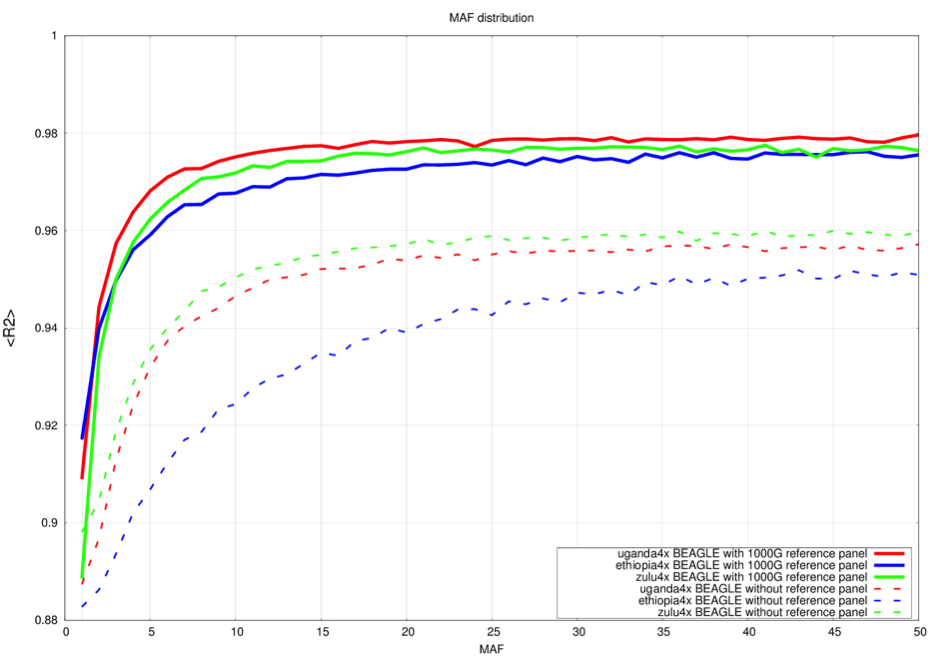
\includegraphics[width=0.75\textwidth]{fig/SN09f3}
\caption{Improvement in imputation accuracy when utilizing a 1000G phase 1 reference panel for each of the 3 sequenced populations.}
\label{fig:SN09f3}
\end{figure}

\paragraph{Evaluation of reference panel upon exclusion of rare variants from it}
A modified 1000G phase reference panel was distributed with Beagle3.\footnote{\url{http://bochet.gcc.biostat.washington.edu/beagle/1000_Genomes.phase1_release_v3}} Rare variants with less than 5 allele counts out of 1092 samples and multiallelic SNPs and indels were removed from the March 2012 release of the Beagle3 distributed 1000G phase 1 reference panel. The low frequency markers were omitted, because genotype errors for low frequency markers in 1000G can possibly affect nearby markers.\footnote{Private correspondence with Brian Browning} We wanted to test this and carried out imputation with the full 1000G phase 1 reference panel and the reduced reference panel distributed with Beagle3. The reduced reference panel was shown to lead to a greater imputation accuracy than the full reference panel (figure \ref{fig:imp_accu_beagle}). Therefore we used the reduced reference panel at the cost of not imputing very rare variants from 1000G phase 1.
\begin{figure}[htbp]
\centering
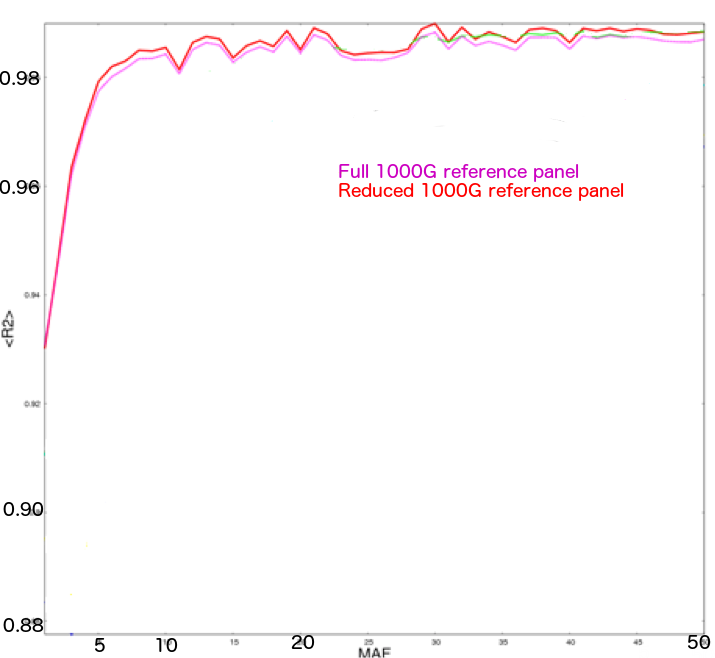
\includegraphics[width=0.66\textwidth]{fig/imp_accu_beagle}
\caption[Comparison of full and reduced reference panel.]{Comparison of full and reduced reference panel. Correlation between the Baganda Omni2.5 genotypes and the Beagle3 refined Baganda HiSeq2000 4x genotypes. The reduced (red) reference panel is the one distributed with Beagle3, which has had multiallelic sites and sites with a minor allele count of 5 removed.}
\label{fig:imp_accu_beagle}
\end{figure}

\paragraph{Evaluation of the best refinement software and sequence of implementation}
To identify the best imputation software and imputation approach we tried out various approaches. In addition to Beagle3 we carried out imputation with IMPUTE2\cite{10.1371/journal.pgen.1000529} with different parameter settings. It has previously been suggested that sequential imputation approaches can increase the accuracy compared to single step imputation.\cite{Pasaniuc2012}
%"We also attempted running MaCH/Thunder starting from results of Beagle but the increase in accuracy was marginal"
We therefore used IMPUTE2 separately and in succession with Beagle3. We used IMPUTE2 with the -{}-pgs\_prob argument, which tells IMPUTE2 to estimate posterior probabilities. We assessed accuracy as correlation with genotypes on the Omni2.5M SNP array. This comparison was only carried out for the 100 Baganda samples sequenced to a 4x coverage, which had been called and filtered separately of the two other populations. We used a truth sensitivity threshold of 96\% for this analysis.
Ultimately we decided that imputation with Beagle3\cite{Browning20071084} using a \gls{1000G} phase 1 reference panel yielded a greater imputation accuracy upon comparison with SNP array genotypes (figures \ref{fig:imp_accu_improv_refiners} \ref{fig:SN09f4}).
\begin{figure}[htbp]
\centering
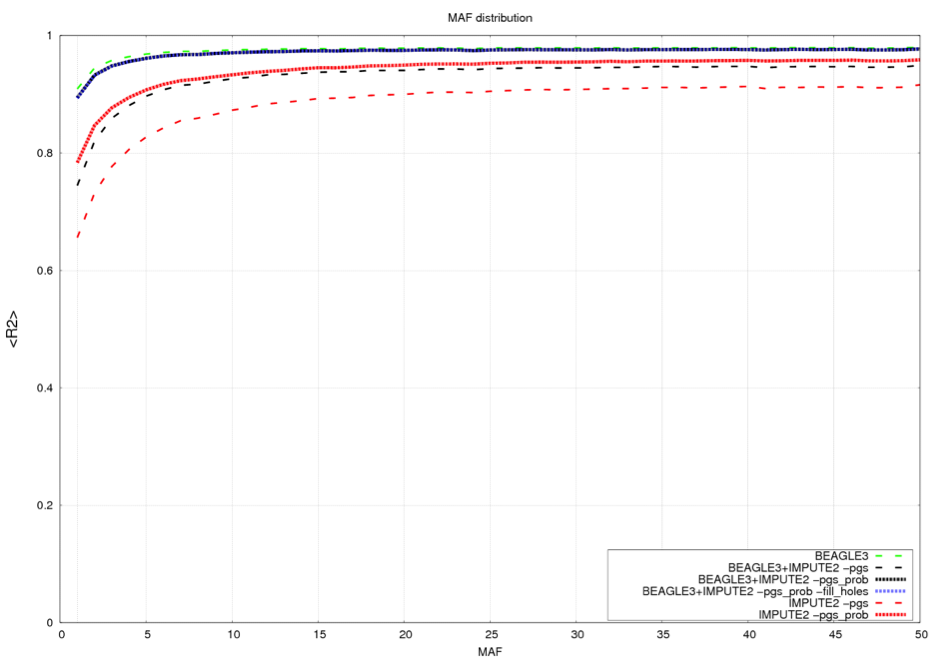
\includegraphics[width=0.75\textwidth]{fig/imp_accu_improv_refiners}
\caption{Comparison of imputation accuracy for the genotypes derived from 4x Baganda sequence data using various imputation strategies.}
\label{fig:imp_accu_improv_refiners}
\end{figure}
\begin{figure}[htbp]
\centering
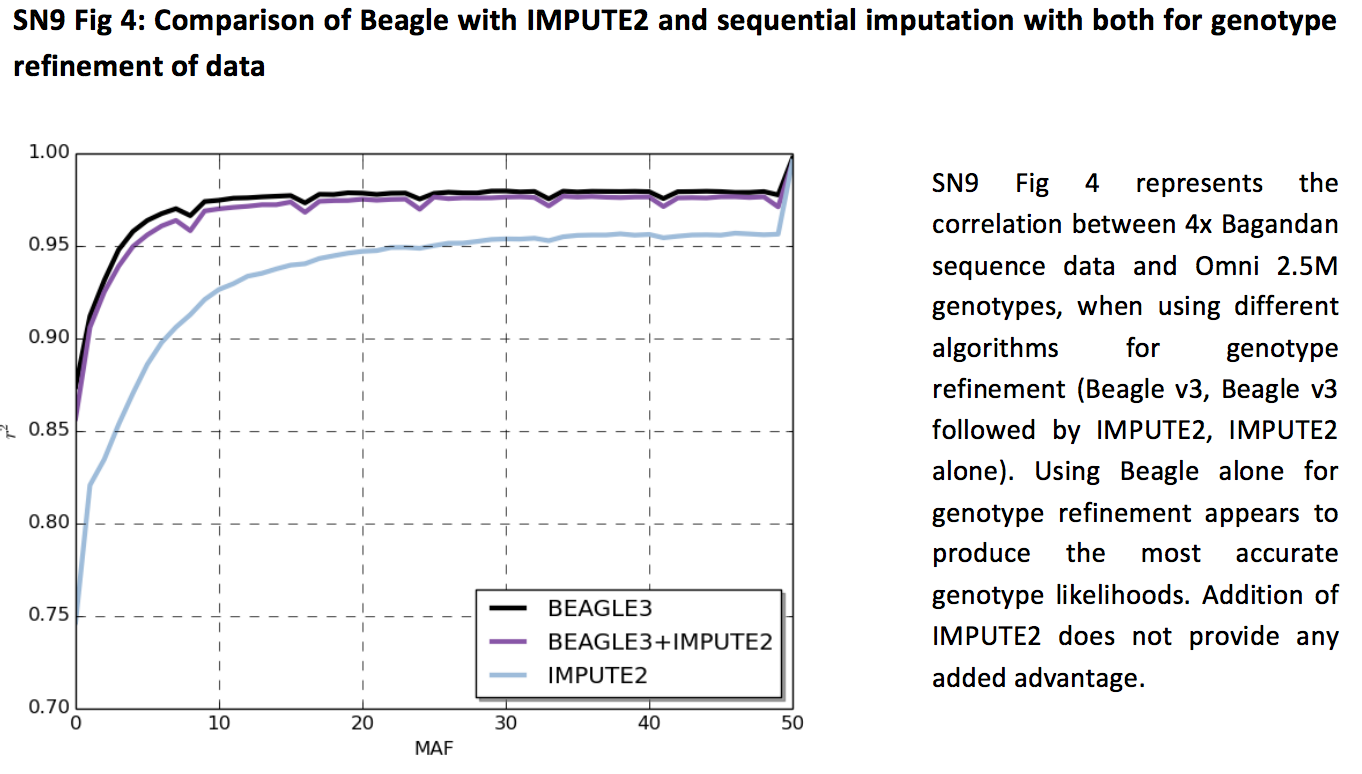
\includegraphics[trim={0 0cm 10cm 2cm},clip,width=0.75\textwidth]{fig/SN09f4}
\caption[Evaluation of refinement strategies.]{Correlation between 4x Bagandan sequence data and Omni2.5M genotypes, when using different algorithms for genotype refinement (Beagle v3\cite{Browning20071084}, Beagle v3 followed by IMPUTE2\cite{10.1371/journal.pgen.1000529}, IMPUTE2 alone). Using Beagle alone for genotype refinement appears to produce the most accurate genotype likelihoods. Addition of IMPUTE2 does not provide any added advantage.}
\label{fig:SN09f4}
\end{figure}

We used an interval size of 2\gls{Mbp} for imputation. Fragments with few variants near centromeres and telomeres and in sparse regions were avoided by not allowing intervals to extend across centromeres and by extension of intervals until containing at least 400\gls{kbp} and 1000 variants. With the exception of fragments next to telomeres and large centromeres, an additional 150\gls{kbp} was included on either side of each fragment to avoid side effects. These fragment edges were not used for any downstream analysis.
We carried out refinement of existing genotype probabilities and inferred missing variants simultaneously despite both the reduced \gls{1000G} phase 1 reference panel and the set of called variants having more than 7\% missing alleles relative to one another. This causes a warning message to appear, but it does not make the refinement inferior and necessitate imputation to be carried out twice; once within the population for novel variants and once with the reference panel for known variants.

\subsubsection{Post-refinement \gls{QC}}
We checked for heterozygosity and \gls{PCA} outliers after refinement, but did not exclude additional samples. Heterozygosity was calculated with GNU Awk\footnote{\url{http://www.gnu.org/software/gawk/manual/gawk.html}} and principal components with Eigensoft4.2\cite{10.1371/journal.pgen.0020190}\cite{Price2006}



\subsection{Comparison of down-sampled data with other study designs}
We evaluated the ability to call genotypes with \gls{ULC} sequence data by comparison to SNP array data for a subset of the samples and the original non-downsampled data by calculation of genotype correlation (page \pageref{subsec:correlation}) and calculation of sensitivity and specificity (page \pageref{subsec:sensspec}) respectively.

\subsubsection{Correlation}
\label{subsec:correlation}
SNP array data was available for a subset of the sequenced samples, and it was therefore possible to evaluate the \gls{ULC} data by comparison of genotypes from each source and calculation of correlations between these.
The calculated correlations are subsequently used to calculate apparent sample sizes at a fixed budget (page \pageref{subsec:samplesize}).
Unless otherwise stated we carried out calculations of correlation as described in this section. Correlation is calculated irrespective of SNP call rate and posterior genotype probabilities using Python\footnote{\url{https://github.com/team149/tc9/blob/master/comparison/correlation.py}}. Hence the correlation is calculated for \glspl{SNP} with high and low imputation quality. Dosages are calculated from the genotype probabilities and correlation is calculated using dosages. The correlation is calculated as a simple average of correlations in each \gls{MAF} bin instead of calculating the correlation for all genotypes for all \glspl{SNP} in each \gls{MAF} bin. The calculation is only carried out for sites that are variant on both the chip and in the sequence data. Hence a correlation will not be calculated, when a monomorphic site is called and refined as a variant site and vice versa. The Omni2.5 \gls{SNP} array has been shown to contain incorrectly genotyped SNPs\cite{Gurdasani2015}, but we cannot predict which ones they are, so we didn't take extra measures to take these into account and remove them from the data set prior to calculation of correlations.

\subsubsection{Sensitivity and specificity}
\label{subsec:sensspec}
The down-sampled data and the SNP array data was compared to the higher coverage data by calculation of sensititivy and specificty (figure \ref{fig:SN12f2}). Sensitivity is the proportion of genotypes in a set of reference high coverage samples, which are correctly called in the calls from the down-sampled data and the SNP array data. Specificity (1 - false positive rate) is the proportion of genotypes in a set of down-sampled samples, which are identical to the reference samples at higher coverage.
The \gls{SNP} array data was compared to the reference sequence data (4x/8x) after imputation with the software IMPUTE2 using the \gls{1000G} phase 1 reference panel.

\begin{figure}
\centering
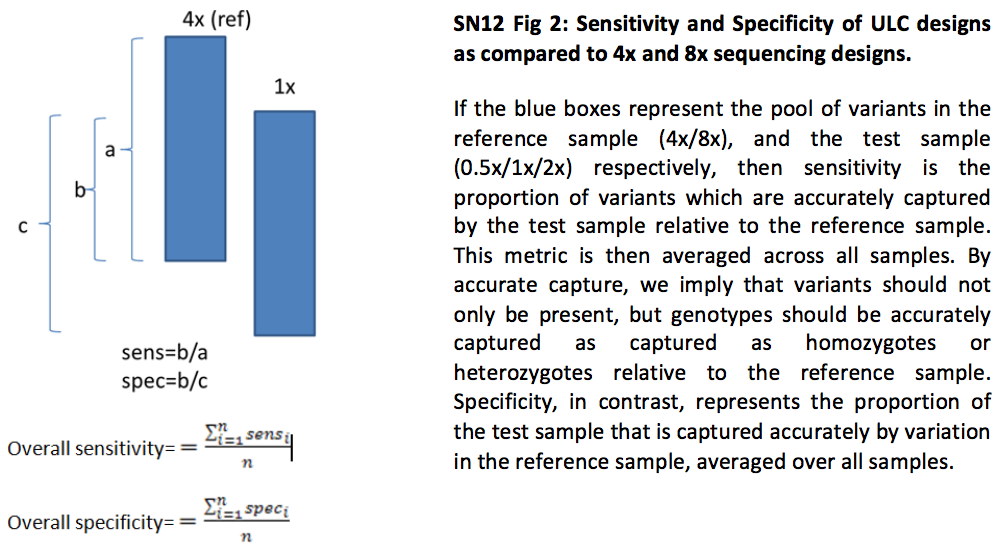
\includegraphics[trim={0 0 0cm 0},clip,width=0.9\textwidth]{fig/SN12f2}
\caption[Sensitivity and specificity as compared between higher and lower coverage sequence data.]{The blue boxes represent the pool of variants in the reference sample (4x/8x), and the test sample (0.5x/1x/2x) respectively. Sensitivity is the proportion of variants which are accurately captured by the test sample relative to the reference sample. This metric is then averaged across all samples. By accurate capture, we imply that variants should not only be present, but genotypes should be accurately captured as homozygous or heterozygous relative to the reference sample. Specificity represents the proportion of the test sample that is captured accurately by variation in the reference sample, averaged over all samples.}
\label{fig:SN12f2}
\end{figure}



\subsection{Calculation of apparent sample sizes}
\label{subsec:samplesize}
To do an assesment of the cost effectivnes of different study designs we want to calculate the apparent sample size at a fixed budget by looking at the coverage that can be obtained for a given study design. We multiply the given sample size by the accuracy of the genotype calling of sequence data to get the apparent sample size. For the calculation of the sample size at a fixed budget the values in table \ref{tab:costs} were used. The total cost  for $n$ number of samples is calculated with equation \ref{eq:sample_size}. The apparent sample size at a given coverage and \gls{MAF} is calculated as the product of the sensitivity at that \gls{MAF} and the cost at that coverage. For the SNP array data the \gls{r2} metric (r\textsuperscript{2}\_typeX) obtained after imputation by means of masking as described in the documentation\footnote{\url{https://mathgen.stats.ox.ac.uk/impute/impute_v2.html}} is used for calculation of apparent sample size. The rare variants in particular might be affected by SNP ascertainment and should therefore be considered upper limits, but the correlations should represent the truth for common variants for which ascertainment is less pronounced.

Computational costs are not included, but assuming a \gls{CPU} hour costs \gls{GBP} 0.17, disk storage is free and no steps are repeated, then the computational cost for 100 samples at 8x is at least \gls{GBP} 1,500. In comparison \gls{SNP} array associated computational costs are negligible and do not require an extensive framework.
\begin{table}[htp]
\centering
\begin{tabular}{l|r}
 & Cost (\gls{GBP}) \\ \hline
Lane & 950.00 \\
Library & 32.50 \\
Omni2.5 & 183.33 \\
\end{tabular}
\caption{Costs associated with sequencing and \gls{SNP} array genotyping.}
\label{tab:costs}
\end{table}

% what are the magic numbers 8 and 4? I forgot...
\begin{equation}
\text{sequencing cost for } n \text{ samples} = \text{lane cost} \times n/(8 \times 4 / \text{coverage}) + n \times \text{library cost}
\label{eq:sample_size}
\end{equation}